\documentclass[aspectratio=169,10pt]{beamer}

\makeatletter
\NeedsTeXFormat{LaTeX2e}
\ProvidesPackage{beamerthemeDUNEProfessional}[2026/08/19 DUNE professional Beamer theme]

\mode<presentation>

\RequirePackage{iftex}
\RequirePackage{graphicx}
\RequirePackage{xcolor}
\RequirePackage{tikz}
\RequirePackage{adjustbox}
\RequirePackage{array}
\RequirePackage{booktabs}
\RequirePackage{tabularx}
\RequirePackage{ragged2e}

\usetikzlibrary{arrows.meta,calc,fit,positioning,shapes.geometric}

\useinnertheme{default}
\useoutertheme{default}
\usefonttheme{professionalfonts}
\setbeamertemplate{navigation symbols}{}

% Logo path is relative to a deck directory. Override with \DuneSetLogoPath.
\newcommand{\DuneLogoPath}{../../templates/dune-professional/logos}
\newcommand{\DuneSetLogoPath}[1]{\renewcommand{\DuneLogoPath}{#1}}

% Color roles. Keep semantic names in decks; avoid ad hoc local colors.
\definecolor{DuneBg}{HTML}{101820}
\definecolor{DunePanel}{HTML}{1B2733}
\definecolor{DunePanelAlt}{HTML}{263645}
\definecolor{DuneTitleBand}{HTML}{20303E}
\definecolor{DuneLine}{HTML}{536878}
\definecolor{DuneText}{HTML}{F1F5F7}
\definecolor{DuneMuted}{HTML}{BAC6CF}
\definecolor{DuneOrange}{HTML}{F2682B}
\definecolor{DuneCyan}{HTML}{8EDDF2}
\definecolor{DuneMint}{HTML}{9BD7AE}
\definecolor{DuneYellow}{HTML}{E8C85A}
\definecolor{DuneRed}{HTML}{F38B7F}
\definecolor{DuneViolet}{HTML}{B8A7E8}

\setbeamercolor{normal text}{fg=DuneText,bg=DuneBg}
\setbeamercolor{title}{fg=white,bg=DuneBg}
\setbeamercolor{subtitle}{fg=DuneMuted,bg=DuneBg}
\setbeamercolor{author}{fg=DuneCyan,bg=DuneBg}
\setbeamercolor{date}{fg=DuneMuted,bg=DuneBg}
\setbeamercolor{frametitle}{fg=white,bg=DuneBg}
\setbeamercolor{headline}{fg=DuneMuted,bg=DuneBg}
\setbeamercolor{footline}{fg=DuneMuted,bg=DuneBg}
\setbeamercolor{itemize item}{fg=DuneOrange}
\setbeamercolor{itemize subitem}{fg=DuneCyan}
\setbeamercolor{enumerate item}{fg=DuneOrange}
\setbeamercolor{caption name}{fg=DuneMuted}

\setbeamercolor{dune panel}{fg=DuneText,bg=DunePanel}
\setbeamercolor{dune panel alt}{fg=DuneText,bg=DunePanelAlt}
\setbeamercolor{dune accent}{fg=DuneBg,bg=DuneCyan}
\setbeamercolor{dune decision}{fg=DuneBg,bg=DuneYellow}
\setbeamercolor{dune risk}{fg=DuneBg,bg=DuneRed}
\setbeamercolor{dune evidence}{fg=DuneBg,bg=DuneMint}
\setbeamercolor{dune violet}{fg=DuneBg,bg=DuneViolet}

\setbeamerfont{normal text}{size=\small}
\setbeamerfont{title}{series=\bfseries}
\setbeamerfont{subtitle}{size=\large}
\setbeamerfont{author}{size=\normalsize,series=\bfseries}
\setbeamerfont{date}{size=\small}
\setbeamerfont{frametitle}{series=\bfseries}
\setbeamerfont{footline}{size=\scriptsize}

\ifPDFTeX
  \RequirePackage[scaled]{helvet}
  \renewcommand*\familydefault{\sfdefault}
  \RequirePackage[T1]{fontenc}
\else
  \RequirePackage{fontspec}
  \defaultfontfeatures{Ligatures=TeX,Scale=MatchLowercase}
  \IfFontExistsTF{IBM Plex Sans}{
    \setsansfont{IBM Plex Sans}
    \setmainfont{IBM Plex Sans}
  }{
    \IfFontExistsTF{Helvetica Neue}{
      \setsansfont{Helvetica Neue}
      \setmainfont{Helvetica Neue}
    }{
      \IfFontExistsTF{TeX Gyre Heros}{
        \setsansfont{TeX Gyre Heros}
        \setmainfont{TeX Gyre Heros}
      }{
        \IfFontExistsTF{Liberation Sans}{
          \setsansfont{Liberation Sans}
          \setmainfont{Liberation Sans}
        }{
          \setsansfont{DejaVu Sans}
          \setmainfont{DejaVu Sans}
        }
      }
    }
  }
  \IfFontExistsTF{JetBrains Mono}{
    \setmonofont{JetBrains Mono}[Scale=0.88]
  }{
    \IfFontExistsTF{Latin Modern Mono}{
      \setmonofont{Latin Modern Mono}[Scale=0.88]
    }{
      \setmonofont{DejaVu Sans Mono}[Scale=0.88]
    }
  }
  \renewcommand*\familydefault{\sfdefault}
\fi

\setbeamersize{text margin left=0.78cm,text margin right=0.78cm}
\setlength{\leftmargini}{1.15em}
\setlength{\leftmarginii}{1.05em}
\setlength{\parskip}{0.18em}

\setbeamertemplate{itemize item}{%
  \color{DuneOrange}\raisebox{0.15ex}{\scriptsize$\blacktriangleright$}%
}
\setbeamertemplate{itemize subitem}{%
  \color{DuneCyan}\raisebox{0.15ex}{\tiny$\blacktriangleright$}%
}

% Measured boxes: content may shrink down, but never expands outside the safe box.
\newcommand{\DuneFitBox}[3]{%
  \begin{adjustbox}{max width=#1,max totalheight=#2}%
    \begin{minipage}{#1}\raggedright #3\end{minipage}%
  \end{adjustbox}%
}

\newcommand{\DuneTightList}{%
  \setlength{\itemsep}{0.45mm}%
  \setlength{\parskip}{0pt}%
}

\newcommand{\DuneEyebrow}[1]{%
  {\color{DuneCyan}\scriptsize\bfseries #1\par}%
}

\newcommand{\DunePill}[2]{%
  \tikz[baseline=-0.55ex]\node[
    rounded corners=2.5pt,
    draw=#1,
    fill=#1!18!DuneBg,
    inner xsep=4pt,
    inner ysep=1.35pt,
    text=#1,
    font=\tiny\bfseries
  ]{#2};%
}

\newcommand{\DuneCard}[4][dune panel]{%
  \begin{beamercolorbox}[wd=\linewidth,sep=5pt,rounded=true]{#1}
    {\usebeamercolor[fg]{#1}\bfseries #2\par}
    \vspace{0.4mm}
    {\usebeamercolor[fg]{#1}\footnotesize #3\par}
    \if\relax\detokenize{#4}\relax\else
      \vspace{0.5mm}{\usebeamercolor[fg]{#1}\scriptsize #4\par}
    \fi
  \end{beamercolorbox}
}

\newcommand{\DuneFixedCard}[5][dune panel]{%
  \begin{beamercolorbox}[wd=\linewidth,sep=5pt,rounded=true]{#1}
    \begin{minipage}[t][#2][t]{\dimexpr\linewidth-10pt\relax}
      \raggedright
      {\usebeamercolor[fg]{#1}\bfseries #3\par}
      \vspace{0.45mm}
      {\usebeamercolor[fg]{#1}\footnotesize #4\par}
      \if\relax\detokenize{#5}\relax\else
        \vspace{0.55mm}{\usebeamercolor[fg]{#1}\scriptsize #5\par}
      \fi
    \end{minipage}
  \end{beamercolorbox}
}

\newcommand{\DuneFooterLogo}{%
  \IfFileExists{\DuneLogoPath/logosolo.png}{%
    \tikz[baseline=-0.52ex]\node[opacity=0.42,inner sep=0pt]{%
      \includegraphics[height=0.25cm]{\DuneLogoPath/logosolo.png}%
    };%
  }{}%
}

\newcommand{\DuneTalkDate}{%
  \@ifundefined{mydate}{\today}{\mydate}%
}

% Background and fixed frame-title band.
\addtobeamertemplate{background canvas}{%
  \begin{tikzpicture}[remember picture,overlay]
    \fill[DuneBg] (current page.south west) rectangle (current page.north east);
    \draw[DuneLine,line width=0.55pt]
      ($(current page.south west)+(0.78,0.74)$)
      -- ($(current page.south east)+(-0.78,0.74)$);
    \fill[DuneCyan!16]
      ($(current page.south east)+(-3.2,0.83)$) rectangle ++(1.45,0.055);
  \end{tikzpicture}%
}{}

\setbeamertemplate{headline}{}

\setbeamertemplate{frametitle}{%
  \nointerlineskip%
  \begin{tikzpicture}[remember picture,overlay]
    \fill[DuneTitleBand]
      (current page.north west) rectangle ($(current page.north east)+(0,-1.18)$);
    \fill[DuneOrange]
      ($(current page.north west)+(0.78,-0.23)$) rectangle ++(1.38,0.055);
    \node[anchor=west,inner sep=0pt]
      at ($(current page.north west)+(0.78,-0.72)$) {%
        \DuneFitBox{\dimexpr\paperwidth-1.56cm\relax}{6.7mm}{%
          {\color{white}\bfseries\fontsize{17}{20}\selectfont\insertframetitle}%
        }%
      };
    \ifx\insertframesubtitle\@empty\else
      \node[anchor=west,inner sep=0pt]
        at ($(current page.north west)+(0.78,-1.02)$) {%
          \DuneFitBox{\dimexpr\paperwidth-1.56cm\relax}{3.2mm}{%
            {\color{DuneMuted}\scriptsize\insertframesubtitle}%
          }%
        };
    \fi
  \end{tikzpicture}%
  \vspace*{12.5mm}%
}

\setbeamertemplate{footline}{%
  \leavevmode%
  \begin{beamercolorbox}[wd=\paperwidth,ht=6.4mm,dp=1.8mm,leftskip=0.78cm,rightskip=0.78cm]{footline}
    \DuneFooterLogo\hspace{0.45em}{\textcolor{DuneMuted}{\DuneTalkDate}}%
    \hfill%
    {\textcolor{DuneOrange}{\bfseries\insertframenumber}\textcolor{DuneMuted}{/\inserttotalframenumber}}%
  \end{beamercolorbox}%
}

\setbeamertemplate{title page}{%
  \begin{tikzpicture}[remember picture,overlay]
    \fill[DuneBg] (current page.south west) rectangle (current page.north east);
    \fill[DuneTitleBand]
      (current page.north west) rectangle ($(current page.north east)+(0,-3.03)$);
    \fill[DuneOrange]
      ($(current page.north west)+(0.82,-0.58)$) rectangle ++(1.55,0.075);
    \fill[DuneCyan]
      ($(current page.south east)+(-2.8,0.79)$) rectangle ++(1.88,0.065);
    \IfFileExists{\DuneLogoPath/DUNElogo_white.png}{%
      \node[anchor=south east,opacity=0.13,inner sep=0pt]
        at ($(current page.south east)+(-0.55,1.42)$) {%
        \includegraphics[width=0.34\paperwidth]{\DuneLogoPath/DUNElogo_white.png}%
      };
    }{}%
    \IfFileExists{\DuneLogoPath/FNAL-Logo-NAL-Light.png}{%
      \node[anchor=south east,inner sep=0pt]
        at ($(current page.south east)+(-0.92,0.78)$) {%
        \includegraphics[height=0.42cm]{\DuneLogoPath/FNAL-Logo-NAL-Light.png}%
      };
    }{}%
    \node[anchor=north west,inner sep=0pt]
      at ($(current page.north west)+(0.82,-0.88)$) {%
        \DuneFitBox{0.78\paperwidth}{1.48cm}{%
          {\color{white}\bfseries\fontsize{25}{28}\selectfont\inserttitle}%
        }%
      };
    \node[anchor=north west,inner sep=0pt]
      at ($(current page.north west)+(0.82,-3.55)$) {%
        \DuneFitBox{0.56\paperwidth}{1.35cm}{%
          {\color{DuneMuted}\fontsize{13}{17}\selectfont\insertsubtitle}%
        }%
      };
    \node[anchor=north west,text=DuneCyan,font=\bfseries,inner sep=0pt]
      at ($(current page.north west)+(0.82,-6.3)$) {\insertauthor};
    \node[anchor=north west,text=DuneMuted,font=\small,inner sep=0pt]
      at ($(current page.north west)+(0.82,-6.82)$) {\insertdate};
  \end{tikzpicture}%
  \vfill%
}

\tikzset{
  dune repo/.style={
    draw=DuneCyan,
    fill=DuneCyan!12!DunePanel,
    text=DuneText,
    rounded corners=3pt,
    align=center,
    text width=2.35cm,
    minimum height=0.86cm,
    inner sep=4pt,
    font=\scriptsize\bfseries
  },
  dune repo muted/.style={
    draw=DuneLine,
    fill=DunePanelAlt,
    text=DuneText,
    rounded corners=3pt,
    align=center,
    text width=2.35cm,
    minimum height=0.86cm,
    inner sep=4pt,
    font=\scriptsize\bfseries
  },
  dune artifact/.style={
    draw=DuneMint,
    fill=DuneMint!13!DunePanel,
    text=DuneText,
    rounded corners=3pt,
    align=center,
    text width=2.35cm,
    minimum height=0.86cm,
    inner sep=4pt,
    font=\scriptsize\bfseries
  },
  dune decision node/.style={
    draw=DuneYellow,
    fill=DuneYellow!14!DunePanel,
    text=DuneText,
    rounded corners=3pt,
    align=center,
    text width=2.35cm,
    minimum height=0.86cm,
    inner sep=4pt,
    font=\scriptsize\bfseries
  },
  dune flow/.style={-Latex,draw=DuneCyan,line width=0.85pt},
  dune relation/.style={draw=DuneMuted,line width=0.65pt},
  dune evidence flow/.style={-Latex,draw=DuneViolet,dashed,line width=0.85pt},
  dune label/.style={
    fill=DuneBg,
    text=DuneMuted,
    inner sep=1.5pt,
    font=\tiny,
    align=center
  }
}

\mode<all>

\makeatother

\title[SC/DPS Git Management]{SC/DPS Git Management}
\subtitle{A clear repository plan around official references, DAQ ZMQ/protobuf interfaces, OPC-UA bridges, safety checks, and release evidence}
\author{Manuel Arroyave}
\date{DUNE slow-controls software discussion -- 20 August 2026}
\newcommand{\mydate}{20 August 2026}
\hypersetup{colorlinks=true,urlcolor=DuneCyan,linkcolor=DuneCyan}
\newcommand{\edmsdoc}[1]{\href{https://edms.cern.ch/document/#1}{\texttt{EDMS #1}}}
\newcommand{\edmsproj}[1]{\href{https://edms.cern.ch/project/#1}{\texttt{EDMS project #1}}}
\newcommand{\ghrepo}[2]{\href{https://github.com/#1/#2}{\nolinkurl{#1/#2}}}

\begin{document}

\begin{frame}[plain]
  \titlepage
\end{frame}

\begin{frame}{Start From Official Sources}
\begin{columns}[T,onlytextwidth]
  \begin{column}{0.54\textwidth}
    \DuneEyebrow{SOURCE OF RECORD}
    \begin{itemize}
      \DuneTightList
      \item Requirements and interfaces come from approved EDMS and official DUNE documents.
      \item Git repositories implement, test, package, and document software behavior against those sources.
      \item Unlinked notes, prototype repos, and slides are evidence or proposals, not authority.
      \item Each production repo should point to the exact official source it implements.
    \end{itemize}
  \end{column}
  \begin{column}{0.42\textwidth}
    \DuneFixedCard[dune decision]{1.35cm}{Practical rule}
      {A production change needs an official reference, a contract version, and evidence that the dependent clients still work.}
      {}
    \vspace{1.5mm}
    \DuneFixedCard[dune evidence]{1.35cm}{Initial references}
      {Use online EDMS/DUNE links only. The next slide is the starter reference register.}
      {}
  \end{column}
\end{columns}
\end{frame}

\begin{frame}{Reference Register We Should Maintain}
\scriptsize
\renewcommand{\arraystretch}{1.12}
\DuneEyebrow{ALL EXAMPLES ARE CLICKABLE ONLINE LINKS}
\vspace{0.7mm}
\begin{tabularx}{\textwidth}{p{0.27\textwidth} p{0.30\textwidth} X}
\toprule
Reference class & Examples & What the Git repos record \\
\midrule
SC/DPS and subsystem ICDs &
\edmsdoc{3309688} (PDS SC), \edmsdoc{3362709} (BDE), \edmsdoc{3315615} (HVS), \edmsdoc{3297045} (TDE), \edmsdoc{3449868} (DAQ), \edmsdoc{2401090} (DPS). &
Which variables, commands, permits, interlocks, and failure behavior are in scope. \\
\addlinespace
HWDB and installation identity &
\edmsproj{CERN-0000279681} (HWDB exports), \edmsdoc{3357086} (PDS to HWDB), rack/network/interface records linked from EDMS. &
How software maps tags and endpoints to real installed identities without duplicating live inventory. \\
\addlinespace
Official software sources &
\ghrepo{DUNE-DAQ}{daphnemodules}, \ghrepo{DUNE-DAQ}{daphne-firmware}, \ghrepo{DUNE-DAQ}{dune-wib-firmware}, canonical board-service repos once chosen. &
Which code owns each producer, consumer, schema, build artifact, and release tag. \\
\addlinespace
Release and evidence records &
System release BOM, VST reports, compatibility matrix, signed or traceable tags. &
Which versions were tested together and what rollback path is approved. \\
\bottomrule
\end{tabularx}
\end{frame}

\begin{frame}{Systems We Are Considering}
\begin{columns}[T,onlytextwidth]
  \begin{column}{0.32\textwidth}
    \DuneFixedCard[dune accent]{2.35cm}{Device producers}
      {DAPHNE and WIB firmware, board services, ZMQ/protobuf actors, GIZMo OPC-UA producer, support-equipment adapters.}
      {\DunePill{DuneCyan}{producer owns truth}}
  \end{column}
  \begin{column}{0.32\textwidth}
    \DuneFixedCard[dune evidence]{2.35cm}{Consumers and projections}
      {DUNE DAQ controllers/opmon, OPC-UA bridges, Ignition Gateway projects, dashboards, archival paths.}
      {\DunePill{DuneMint}{same contract}}
  \end{column}
  \begin{column}{0.32\textwidth}
    \DuneFixedCard[dune decision]{2.35cm}{Verification and deployment}
      {Fleet emulator, vertical-slice tests, release BOM, host services, network/port policy, rollback procedure.}
      {\DunePill{DuneYellow}{tested set}}
  \end{column}
\end{columns}
\vspace{3mm}
\DuneCard[dune panel alt]{Boundary statement}
  {The repository plan follows these interfaces. It is not a proposal to merge all code into one repository or to replace existing DUNE-DAQ ownership.}
  {}
\end{frame}

\begin{frame}{Why This Organization}
\begin{columns}[T,onlytextwidth]
  \begin{column}{0.48\textwidth}
    \DuneEyebrow{THE PROBLEM}
    \begin{itemize}
      \DuneTightList
      \item DAQ and SC both talk to board services, often through the same ZMQ/protobuf contracts.
      \item Bridges can accidentally carry private schema copies and drift from DAQ behavior.
      \item Firmware, board services, bridges, Ignition exports, and deployment do not release on the same cadence.
      \item Safety-related assumptions can be hidden in code unless they are tracked as explicit gates.
    \end{itemize}
  \end{column}
  \begin{column}{0.48\textwidth}
    \DuneEyebrow{THE ORGANIZATION}
    \begin{itemize}
      \DuneTightList
      \item Put contracts and compatibility policy where everyone can review them.
      \item Keep device implementation beside the teams that own the device behavior.
      \item Put cross-system tests and release BOMs in a place whose job is integration evidence.
      \item Keep secrets and site-specific runtime values outside public Git.
    \end{itemize}
  \end{column}
\end{columns}
\end{frame}

\begin{frame}{System and Interface Map}
\centering
\begin{adjustbox}{max width=\textwidth,max totalheight=0.72\textheight,center}
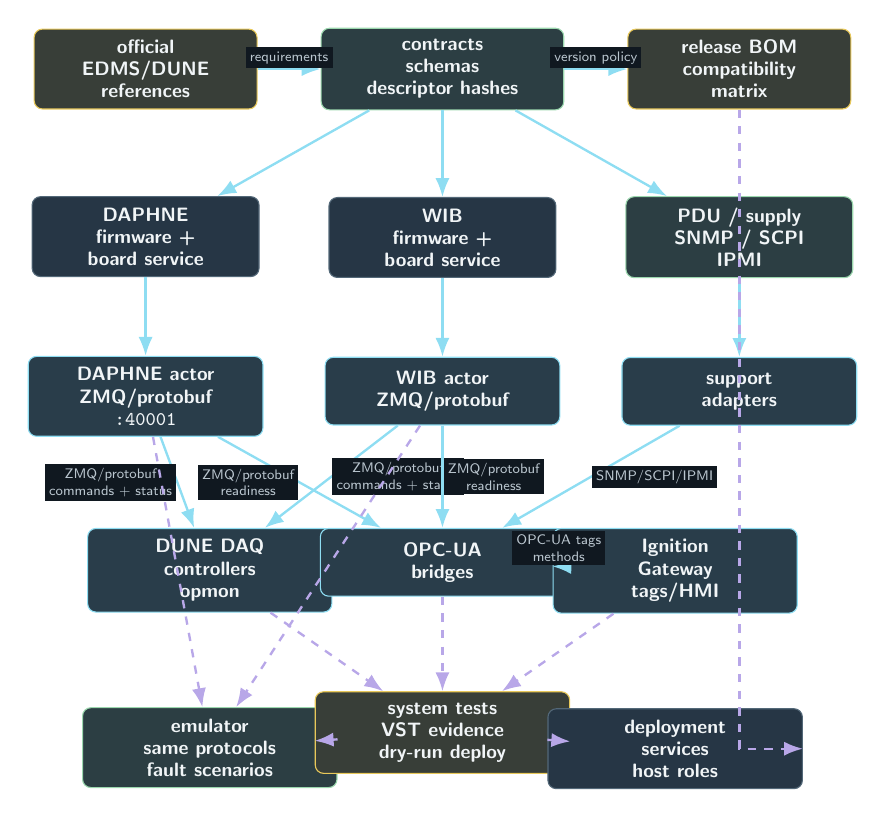
\begin{tikzpicture}[node distance=7mm and 8mm]
  \node[dune decision node,text width=2.55cm] (refs) {official\\EDMS/DUNE\\references};
  \node[dune artifact,text width=2.80cm,right=of refs] (contracts) {contracts\\schemas\\descriptor hashes};
  \node[dune decision node,text width=2.55cm,right=of contracts] (bom) {release BOM\\compatibility\\matrix};

  \node[dune repo muted,text width=2.60cm,below=11mm of refs] (daphnefw) {DAPHNE\\firmware +\\board service};
  \node[dune repo muted,text width=2.60cm,below=11mm of contracts] (wibfw) {WIB\\firmware +\\board service};
  \node[dune artifact,text width=2.60cm,below=11mm of bom] (support) {PDU / supply\\SNMP / SCPI\\IPMI};

  \node[dune repo,text width=2.70cm,below=10mm of daphnefw] (daphnezmq) {DAPHNE actor\\ZMQ/protobuf\\\texttt{:40001}};
  \node[dune repo,text width=2.70cm,below=10mm of wibfw] (wibzmq) {WIB actor\\ZMQ/protobuf};
  \node[dune repo,text width=2.70cm,below=10mm of support] (supportadapter) {support\\adapters};

  \node[dune repo,text width=2.82cm,below left=13mm and -1mm of wibzmq] (daq) {DUNE DAQ\\controllers\\opmon};
  \node[dune repo,text width=2.82cm,below=13mm of wibzmq] (opcua) {OPC-UA\\bridges};
  \node[dune repo,text width=2.82cm,below right=13mm and -1mm of wibzmq] (ignition) {Ignition\\Gateway\\tags/HMI};

  \node[dune artifact,text width=2.95cm,below=12mm of daq] (emu) {emulator\\same protocols\\fault scenarios};
  \node[dune decision node,text width=2.95cm,below=12mm of opcua] (tests) {system tests\\VST evidence\\dry-run deploy};
  \node[dune repo muted,text width=2.95cm,below=12mm of ignition] (deploy) {deployment\\services\\host roles};

  \draw[dune flow] (refs) -- node[dune label,above] {requirements} (contracts);
  \draw[dune flow] (contracts) -- node[dune label,above] {version policy} (bom);
  \draw[dune flow] (contracts) -- (daphnefw);
  \draw[dune flow] (contracts) -- (wibfw);
  \draw[dune flow] (contracts) -- (support);
  \draw[dune flow] (daphnefw) -- (daphnezmq);
  \draw[dune flow] (wibfw) -- (wibzmq);
  \draw[dune flow] (support) -- (supportadapter);

  \draw[dune flow] (daphnezmq) -- node[dune label,left] {ZMQ/protobuf\\commands + status} (daq);
  \draw[dune flow] (wibzmq) -- node[dune label,right] {ZMQ/protobuf\\commands + status} (daq);
  \draw[dune flow] (daphnezmq) -- node[dune label,left] {ZMQ/protobuf\\readiness} (opcua);
  \draw[dune flow] (wibzmq) -- node[dune label,right] {ZMQ/protobuf\\readiness} (opcua);
  \draw[dune flow] (supportadapter) -- node[dune label,right] {SNMP/SCPI/IPMI} (opcua);
  \draw[dune flow] (opcua) -- node[dune label,above] {OPC-UA tags\\methods} (ignition);

  \draw[dune evidence flow] (daphnezmq) -- (emu);
  \draw[dune evidence flow] (wibzmq) -- (emu);
  \draw[dune evidence flow] (emu) -- (tests);
  \draw[dune evidence flow] (daq) -- (tests);
  \draw[dune evidence flow] (opcua) -- (tests);
  \draw[dune evidence flow] (ignition) -- (tests);
  \draw[dune evidence flow] (deploy) -- (tests);
  \draw[dune evidence flow] (bom) |- (deploy);
\end{tikzpicture}
\end{adjustbox}
\end{frame}

\begin{frame}{What We Need to Track}
\scriptsize
\renewcommand{\arraystretch}{1.13}
\begin{tabularx}{\textwidth}{p{0.23\textwidth} p{0.32\textwidth} X}
\toprule
Thing to track & Minimum record & Why it matters \\
\midrule
Official reference &
EDMS/DUNE document ID, revision, owner, interpreted scope. &
Prevents local assumptions from becoming silent requirements. \\
\addlinespace
Contract identity &
Schema version, descriptor hash, producer repo/tag, compatible consumers. &
Makes DAQ, bridge, emulator, and deployment compatibility reviewable. \\
\addlinespace
Command authority &
Who may write in each lifecycle state, stale limits, rejection behavior, audit fields. &
Prevents DAQ/SC races and makes unsupported writes fail closed. \\
\addlinespace
Safety assumptions &
Permit source, interlock owner, failure survival claim, reset/rollback path. &
Prevents monitoring software from being credited with independent protection. \\
\addlinespace
Evidence &
CI logs, emulator scenarios, one-board vertical-slice results, release BOM. &
Shows the selected versions worked together before deployment. \\
\bottomrule
\end{tabularx}
\end{frame}

\begin{frame}{Safety and Dependency Checks in Git}
\begin{columns}[T,onlytextwidth]
  \begin{column}{0.48\textwidth}
    \DuneFixedCard[dune risk]{2.45cm}{Safety checks}
      {No secrets or site credentials. Writes gated by lifecycle and fresh permits. Unsafe command paths fail closed. DPS/protection claims require the designated owner and evidence that the action survives the initiating failure.}
      {}
  \end{column}
  \begin{column}{0.48\textwidth}
    \DuneFixedCard[dune evidence]{2.45cm}{Dependency checks}
      {Schema hash compatibility. Producer/consumer matrix. Emulator scenario with real DAQ ZMQ client and real OPC-UA bridge. Release BOM validated before deployment.}
      {}
  \end{column}
\end{columns}
\vspace{3mm}
\DuneCard[dune panel alt]{Review gate}
  {A contract-changing pull request should link the official reference, affected producers, DAQ consumers, bridges, emulator scenarios, deployment impact, test evidence, and rollback plan.}
  {}
\end{frame}

\begin{frame}{Repository Roles}
\scriptsize
\renewcommand{\arraystretch}{1.12}
\begin{adjustbox}{max width=\textwidth,max totalheight=0.70\textheight,center}
\begin{tabularx}{\textwidth}{>{\bfseries\ttfamily}p{0.25\textwidth} p{0.30\textwidth} X}
\toprule
Repo role & Owns & Does not own \\
\midrule
scdps-coordination &
Reference register, matrix, ADRs, RACI, release compatibility table. &
Device implementation or live inventory. \\
\addlinespace
scdps-contracts &
Common status semantics, schema policy, descriptor publication, compatibility tooling. &
Every device register or every command. \\
\addlinespace
daphne-sc-service / wib service &
Board actor behavior, ZMQ/protobuf producer, firmware/service readiness. &
Ignition project resources or cross-system release evidence. \\
\addlinespace
daphne-opcua-bridge / wib-opcua-bridge &
Device-specific OPC-UA mappings, quality/staleness, methods, bridge tests. &
Private schema forks or independent protection decisions. \\
\addlinespace
scdps-emulator &
Production-like protocol behavior, fault scenarios, protocol-source pinning. &
Production HMI or production DPS logic. \\
\addlinespace
scdps-system-tests / deployment &
VST orchestration, evidence reports, release BOM, host services, rollback. &
Secrets, live operational databases, or HWDB duplication. \\
\bottomrule
\end{tabularx}
\end{adjustbox}
\end{frame}

\begin{frame}{Adoption Path}
\centering
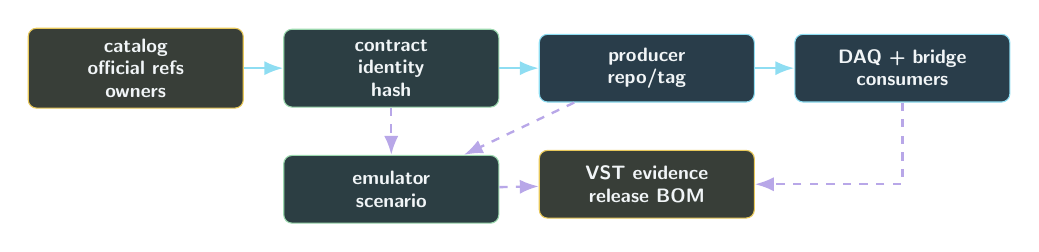
\begin{tikzpicture}[node distance=6mm and 5mm]
  \node[dune decision node,text width=2.45cm] (catalog) {catalog\\official refs\\owners};
  \node[dune artifact,text width=2.45cm,right=of catalog] (contract) {contract\\identity\\hash};
  \node[dune repo,text width=2.45cm,right=of contract] (producer) {producer\\repo/tag};
  \node[dune repo,text width=2.45cm,right=of producer] (consumers) {DAQ + bridge\\consumers};
  \node[dune artifact,text width=2.45cm,below=of contract] (emu) {emulator\\scenario};
  \node[dune decision node,text width=2.45cm,below=of producer] (evidence) {VST evidence\\release BOM};

  \draw[dune flow] (catalog) -- (contract);
  \draw[dune flow] (contract) -- (producer);
  \draw[dune flow] (producer) -- (consumers);
  \draw[dune evidence flow] (contract) -- (emu);
  \draw[dune evidence flow] (producer) -- (emu);
  \draw[dune evidence flow] (consumers) |- (evidence);
  \draw[dune evidence flow] (emu) -- (evidence);
\end{tikzpicture}

\vspace{3mm}
\DuneCard[dune panel alt]{Online candidates to classify}
  {\ghrepo{marroyav}{daphne_slow_controls_plan}, \ghrepo{marroyav}{daphne-sc}, \ghrepo{ecristal}{daphneZMQ}, \ghrepo{BenLand100}{wib_opcua}, \ghrepo{marroyav}{sc_emu}, \ghrepo{marroyav}{sc_interface}, \ghrepo{marroyav}{GIZMo}, \ghrepo{marroyav}{gizmo-ignition}.}
  {}
\end{frame}

\begin{frame}{Decisions for Thursday}
\begin{columns}[T,onlytextwidth]
  \begin{column}{0.54\textwidth}
    \begin{itemize}
      \DuneTightList
      \item Where is the governed namespace: DUNE, DUNE-DAQ, or a coordinated cross-organization collection?
      \item Which repository owns the canonical DAPHNE and WIB ZMQ/protobuf contracts?
      \item Who are the first CODEOWNERS for references, contracts, DAQ interfaces, bridges, deployment, and evidence?
      \item Which vertical slice proves the first DAQ ZMQ client plus OPC-UA bridge path?
      \item What branch protection, tag, and release-BOM policy is the minimum before wider onboarding?
    \end{itemize}
  \end{column}
  \begin{column}{0.42\textwidth}
    \DuneFixedCard[dune decision]{1.55cm}{Meeting output}
      {Approve the catalog structure and name the owners for the first two contracts.}
      {}
    \vspace{1.5mm}
    \DuneFixedCard[dune evidence]{1.55cm}{First technical proof}
      {Run one DAQ ZMQ client and one OPC-UA bridge against the same emulator scenario in CI.}
      {}
  \end{column}
\end{columns}
\end{frame}

\end{document}
